\documentclass{article}
\usepackage{cmap}
\usepackage[utf8]{inputenc}
\usepackage[english,ukrainian]{babel}
\usepackage{graphicx}
\usepackage{geometry}
\usepackage{listings}
\usepackage{indentfirst}
\usepackage{subfigure}
\usepackage{caption}
\usepackage{amsmath}
\geometry{
	a4paper,
	left=20mm,
	right=20mm,
	top=20mm,
	bottom=20mm
}
\lstset{
	tabsize=4,
	language=python,
	showstringspaces=false,
	showtabs=false,
	frame=lrtb,
	columns=fixed,
	keepspaces,
	breaklines=true,
	extendedchars=\true,
	escapeinside={\%*}{*)}
}
\graphicspath{ {pictures} }
\setlength{\parindent}{4em}
\newcommand\subject{Чисельні методи}
\newcommand\lecturer{доцент кафедри ПЗ\\Мельник Н.Б.}
\newcommand\teacher{асистент кафедри ПЗ\\Гарматій Г.Ю.}
\newcommand\mygroup{ПЗ-16}
\newcommand\lab{5}
\newcommand\theme{Наближені методи розв’язування систем лінійних алгебраїчних рівнянь}
\newcommand\purpose{Ознайомлення на практиці з методами Якобі та Зейделя
	розв’язування систем лінійних алгебраїчних рівнянь}

\begin{document}
	\begin{large}
		\begin{titlepage}
			\thispagestyle{empty}
			\begin{center}
				\textbf{МІНІСТЕРСТВО ОСВІТИ І НАУКИ УКРАЇНИ\\
					НАЦІОНАЛЬНИЙ УНІВЕРСИТЕТ "ЛЬВІВСЬКА ПОЛІТЕХНІКА"}
			\end{center}
			\begin{flushright}
				Інститут \textbf{КНІТ}\\
				Кафедра \textbf{ПЗ}
			\end{flushright}
			\vspace{200pt}
			\begin{center}
				\textbf{ЗВІТ}\\
				\vspace{10pt}
				До лабораторної роботи № \lab\\
				\textbf{На тему}: “\textit{\theme}”\\
				\textbf{З дисципліни}: “\subject”
			\end{center}
			\vspace{90pt}
			\begin{flushright}
				
				\textbf{Лектор}:\\
				\lecturer\\
				\vspace{28pt}
				\textbf{Виконав}:\\
				
				студент групи \mygroup\\
				Коваленко Д.М.\\
				\vspace{28pt}
				\textbf{Прийняв}:\\
				
				\teacher\\
				
				\vspace{28pt}
				«\rule{1cm}{0.15mm}» \rule{1.5cm}{0.15mm} 2022 р.\\
				$\sum$ = \rule{1cm}{0.15mm}……………\\
				
			\end{flushright}
			\vspace{\fill}
			\begin{center}
				\textbf{Львів — 2022}
			\end{center}
		\end{titlepage}
		
		\begin{description}
			\item[Тема.] \theme.
			\item[Мета.] \purpose.
		\end{description}
		
		\section*{Теоретичні відомості}
		\subsection*{Метод Якобі}
		Розглянемо систему лінійних алгебраїчних рівнянь:
		\begin{gather}
			\left\{\begin{array}{@{}l@{}}
				a_{11}x_1 + a_{12}x_2 + \alpha_{13}x_3 + ... + a_{1n}x_n = b_{1},\\\nonumber
				a_{21}x_1 + a_{22}x_2 + \alpha_{23}x_3 + ... + a_{2n}x_n = b_{2},\\\nonumber
				.................................................\\\nonumber
				a_{n1}x_1 + a_{n2}x_2 + \alpha_{n3}x_3 + ... + a_{nn}x_n = b_{n}.\nonumber
			\end{array}\right.\,
		\end{gather}
	
		Припустивши, що коефіцієнти $a_{ii}\ne0\hspace{14pt}(i=\overline{1,n})$, розв’яжемо $i$-те рівняння системи відносноi $x_i$ та введемо позначення:
		\begin{gather}
			\beta_i=\frac{b_i}{a_{ii}}, \hspace{14pt}a_{ij}=-\frac{a_{ij}}{a_{ii}}, \hspace{14pt}i=\overline{1,n}, \hspace{14pt}j\ne i\nonumber
		\end{gather}
	
		Отримаємо:
		\begin{gather}
			\left\{\begin{array}{@{}l@{}}
				x_1 = \beta_1 + \alpha_{12}x_2 + \alpha_{13}x_3+ ... + \alpha_{1n}x_n,\\\nonumber
				x_2 = \beta_2 + \alpha_{21}x_1 + \alpha_{23}x_3 + ... + a_{2n}x_n,\\\nonumber
				.................................................\\\nonumber
				x_n = \beta_n + \alpha_{n2}x_2 + \alpha_{n3}x_3 + ... + a_{nn}x_n.\nonumber
			\end{array}\right.\,
		\end{gather}
	
		Ітераційні формули мають вигляд:
		\begin{gather}
			\left\{\begin{array}{@{}l@{}}
				x_i^{(0)}=\beta_i,\\\nonumber
				x_i^{(k)}=\beta_i+\sum_{j=1}^{i-1}a_{ij}x_j^{(k-1)}+\sum_{j=i+1}^{n}a_{ij}x_j^{(k-1)},\hspace{14pt}i=\overline{1,n}, \hspace{14pt}k=1,2...\nonumber
			\end{array}\right.\,
		\end{gather}
	
		\subsection*{Метод Зейделя}
		Основна відмінність методу Зейделя від методу Якобі полягає в тому, що для обчислення чергового наближення розв’язку використовуються вже знайдені значення.
		
		Ітераційні формули мають вигляд:
		\begin{gather}
			\left\{\begin{array}{@{}l@{}}
				x_i^{(0)}=\beta_i,\\\nonumber
				x_i^{(k)}=\beta_i+\sum_{j=1}^{i-1}a_{ij}x_j^{(k-1)}+\sum_{j=i+1}^{n}a_{ij}x_j^{(k-1)},\hspace{14pt}i=\overline{1,n}, \hspace{14pt}k=1,2...\nonumber
			\end{array}\right.\,
		\end{gather}
		
		\subsection*{Збіжність ітераційного процесу}
		Якщо елементи матриці $\alpha$ системи рівнянь задовольняють одну з умов:
		\begin{gather}\nonumber
			\sum_{j=1}^{n}|\frac{a_{ij}}{a_{ii}}|<1,\hspace{14pt} i=\overline{1,n}\\\nonumber
			\sum_{i=1}^{n}|\frac{a_{ij}}{a_{ii}}|<1,\hspace{14pt} j=\overline{1,n}\\\nonumber
			\sum_{i,j=1}^{n}(\frac{a_{ij}}{a_{ii}})^2<1.\nonumber
		\end{gather}
		то система рівнянь має єдиний розв'язок $X^*$, який не залежить від
		початкового наближення $X^{(0)}$.
		
		\subsection*{Критерії припинення ітераційного процесу}
		Якщо задана похибка $\epsilon$ наближеного розв’язку, то критерієм припинення
		ітераційного процесу вважають виконання однієї з умов:
		\begin{gather}\nonumber
			|X^{(k)}-X^{(k-1)}|=\sqrt{\sum_{i=1}^{n}(x_i^{(k)}-x_i^{(k-1)})^2}<\epsilon,\hspace{14pt}k=1,2...\\\nonumber
			max|x_i^{(k)}-x_i^{(k-1)}|<\epsilon,\hspace{14pt}i=\overline{1,n},\hspace{14pt}k=1,2...\\\nonumber
			max|\frac{x_i^{(k)}-x_i^{(k-1)}}{x_i^{(k)}}|<\epsilon,\hspace{14pt}|x_i|>>1,\hspace{14pt}i=\overline{1,n},\hspace{14pt}k=1,2...
		\end{gather}
		
		\section*{Лабораторне завдання}
		Розв’язати систему лінійних алгебраїчних рівнянь методом Зейделя та
		методом Якобі з точністю $\epsilon=0.001$. Порівняти кількість ітерацій для обох
		методів.
		\begin{gather}\nonumber
			\left\{\begin{array}{@{}l@{}}
				0.65x_1-0.06x_2-0.12x_3+0.14x_4=2.17\\\nonumber
				0.04x_1-0.82x_2+0.08x_3+0.11x_4=-1.14\\\nonumber
				0.34x_1+0.08x_2-0.66x_3+0.14x_4=2.1\\\nonumber
				0.11x_1+0.12x_2\hspace{48pt}-0.53x_4=-0.58\nonumber
			\end{array}\right.\,
		\end{gather}
		\section*{Хід роботи}
		\subsection*{Метод Якобі}	
		\begin{gather}
			\left\{\begin{array}{@{}l@{}}
				0.65x_1-0.06x_2-0.12x_3+0.14x_4=2.17\\\nonumber
				0.04x_1-0.82x_2+0.08x_3+0.11x_4=-1.14\\\nonumber
				0.34x_1+0.08x_2-0.66x_3+0.14x_4=2.1\\\nonumber
				0.11x_1+0.12x_2\hspace{48pt}-0.53x_4=-0.58\nonumber
			\end{array}\right.\,
		\end{gather}
	
		Перепишу систему у зведеному вигляді:
		\begin{gather}
			\left\{\begin{array}{@{}l@{}}
				x_1=3.33+0.09x_2+0.18x_3-0.21x_4\\\nonumber
				x_2=1.39+0.04x_1+0.09x_3+0.13x_4\\\nonumber
				x_3=-3.18+0.51x_1+0.12x_2+0.21x_4\\\nonumber
				x_4=1.09+0.20x_1+0.22x_2\nonumber
			\end{array}\right.\,
		\end{gather}
	
		Звідси:
		\begin{gather}
			\alpha=\begin{pmatrix}
				0 & 0.09 & 0.18 & -0.21\\
				0.04 & 0 & 0.09 & 0.13\\
				0.51 & 0.12 & 0 & 0.21\\
				0.20 & 0.22 & 0 & 0
			\end{pmatrix}\nonumber\hspace{28pt}
			\beta=\begin{pmatrix}
				3.33\\
				1.39\\
				-3.18\\
				1.09
			\end{pmatrix}\nonumber
		\end{gather}
	
		Достатня умова збіжності методу простої ітерації виконується:
		\begin{gather}\nonumber
			\max\{|0.09|+|0.18|+|-0.21|,|0.04|+|0.09|+|0.13|,|0.51|+|0.12|+|0.21|,|0.20|+|0.22|\}=\\\nonumber=\max\{0.48,0.26,0.82,0.42\}=0.82<1\nonumber
		\end{gather}
	
		За початкове наближення візьму стовпець вільних членів $\beta$:
		\begin{gather}
			\left\{\begin{array}{@{}l@{}}
				x_1=3.33\\\nonumber
				x_2=1.39\\\nonumber
				x_3=-3.18\\\nonumber
				x_4=1.09\nonumber
			\end{array}\right.\,
		\end{gather}
	
		Перший крок ітераційного процесу:
		\begin{gather}
			\left\{\begin{array}{@{}l@{}}
				x_1=3.33+0.09\cdot1.39+0.18\cdot(-3.18)-0.21\cdot1.09\\\nonumber
				x_2=1.39+0.04\cdot3.33+0.09\cdot(-3.18)+0.13\cdot1.09\\\nonumber
				x_3=-3.18+0.51\cdot3.33+0.12\cdot1.39+0.21\cdot1.09\\\nonumber
				x_4=1.09+0.20\cdot3.33+0.22\cdot1.39\nonumber
			\end{array}\right.\,\hspace{28pt}
			\left\{\begin{array}{@{}l@{}}
				x_1=2.64\\\nonumber
				x_2=1.38\\\nonumber
				x_3=-1.06\\\nonumber
				x_4=2.10\nonumber
			\end{array}\right.\,
		\end{gather}
	
		Другий крок ітераційного процесу:
		\begin{gather}
			\left\{\begin{array}{@{}l@{}}
				x_1=3.33+0.09\cdot1.38+0.18\cdot(-1.06)-0.21\cdot2.10\\\nonumber
				x_2=1.39+0.04\cdot2.64+0.09\cdot(-1.06)+0.13\cdot2.10\\\nonumber
				x_3=-3.18+0.51\cdot2.64+0.12\cdot1.38+0.21\cdot2.10\\\nonumber
				x_4=1.09+0.20\cdot2.64+0.22\cdot1.38\nonumber
			\end{array}\right.\,\hspace{28pt}
				\left\{\begin{array}{@{}l@{}}
				x_1=2.81\\\nonumber
				x_2=1.69\\\nonumber
				x_3=-1.20\\\nonumber
				x_4=1.95\nonumber
			\end{array}\right.\,\\
		...\nonumber
		\end{gather}
	
		Результат після кількох додаткових ітерацій:
		\begin{gather}
			\left\{\begin{array}{@{}l@{}}
				x_1=2.85\\\nonumber
				x_2=1.70\\\nonumber
				x_3=-1.06\\\nonumber
				x_4=2.07\nonumber
			\end{array}\right.\,
		\end{gather}
		\noindent\textit{\textbf{Код програми} (файл lab\_\lab1.py):}
		\begin{lstlisting}
import numpy as np

def data_to_matrix(path):
	return (
		np.loadtxt(open(path,"rb"),delimiter=",",usecols=[0,1,2,3]),
		np.loadtxt(open(path,"rb"),delimiter=",",usecols=4),
	)

def jacobi_method(A, B, eps):
    """ Метод Якобі """
	print(jacobi_method.__doc__)
	D = np.diag(A)
	a = np.array([-(A - np.diagflat(D))[i] / D[i] for i in range(np.shape(A)[0])])    # %*$\alpha$*)
	b = B / D        # %*$\beta$*)
	
	print(f"%*$\alpha$*):\n {a}\n %*$\beta$*):\n {b}")
	
	X = b.copy() # Початкове наближення
	
	for i in range(10):
		print(f"\tІтерація {i}: {X}")
		X_new = b + np.dot(a, X)
		if np.allclose(X_new, X, atol=eps):
			break
		X = X_new.copy()
	print(f"Відповідь: {X}")

path = input("Введіть шлях до файлу з даними: ") or "data.csv"
A, B = data_to_matrix(path)     # A - матриця коефіцієнтів системи
jacobi_method(A, B, 0.001)      # B - матриця вільних членів\end{lstlisting}
		
		\subsection*{Метод Зейделя}
		Основна відмінність методу Зейделя від методу Якобі полягає в тому, що для обчислення чергового наближення розв’язку використовуються вже знайдені значення.
		
		Перший крок ітераційного процесу:
		\begin{gather}
			\left\{\begin{array}{@{}l@{}}
				x_1=3.33+0.09\cdot1.39+0.18\cdot(-3.18)-0.21\cdot1.09=\textbf{2.64}\\\nonumber
				x_2=1.39+0.04\cdot\textbf{2.64}+0.09\cdot(-3.18)+0.13\cdot1.09=\textbf{1.38}\\\nonumber
				x_3=-3.18+0.51\cdot\textbf{2.64}+0.12\cdot\textbf{1.38}+0.21\cdot1.09=\textbf{-1.06}\\\nonumber
				x_4=1.09+0.20\cdot\textbf{2.64}+0.22\cdot\textbf{1.38}=\textbf{2.10}\nonumber
			\end{array}\right.\,
		\end{gather}
	
		Другий крок ітераційного процесу:
		\begin{gather}
			\left\{\begin{array}{@{}l@{}}
				x_1=3.33+0.09\cdot1.38+0.18\cdot(-1.06)-0.21\cdot2.10=\textbf{2.81}\\\nonumber
				x_2=1.39+0.04\cdot\textbf{2.81}+0.09\cdot(-1.06)+0.13\cdot2.10=\textbf{1.69}\\\nonumber
				x_3=-3.18+0.51\cdot\textbf{2.81}+0.12\cdot\textbf{1.69}+0.21\cdot2.10=\textbf{-1.20}\\\nonumber
				x_4=1.09+0.20\cdot\textbf{2.81}+0.22\cdot\textbf{1.69}=\textbf{1.95}\nonumber
			\end{array}\right.\,\\\nonumber
			...\nonumber
		\end{gather}
		\noindent\textit{\textbf{Код програми} (файл lab\_\lab2.py):}
		\begin{lstlisting}
import numpy as np

def data_to_matrix(path):
	return (
		np.loadtxt(open(path,"rb"),delimiter=",",usecols=[0,1,2,3]),
		np.loadtxt(open(path,"rb"),delimiter=",",usecols=4),
	)

def seidel_method(A, B, eps):
	""" Метод Зейделя """
	print(seidel_method.__doc__)
	X = B / np.diag(A) # Початкове наближення
	
	for i in range(1000):
		print(f"\tІтерація {i}: {X}")
		X_prev = X.copy()
		for k in range(A.shape[0]):
			X[k] = (B[k] - np.dot(A[k, :k], X[:k]) - np.dot(A[k, k+1:], X_prev[k+1:])) / A[k, k]
			if np.allclose(X, X_prev, atol=eps):
				break
	print(f"Відповідь: {X}")

path = input("Введіть шлях до файлу з даними: ") or "data.csv"
A, B = data_to_matrix(path)     # A - матриця коефіцієнтів системи
seidel_method(A, B, 0.001)      # B - матриця вільних членів\end{lstlisting}
		
		\begin{figure}[h!]
			\centering
			\subfigure[]{\includegraphics[width=0.9\textwidth]{1}}\\
			\subfigure[]{\includegraphics[width=0.9\textwidth]{2}}\\
			\subfigure[]{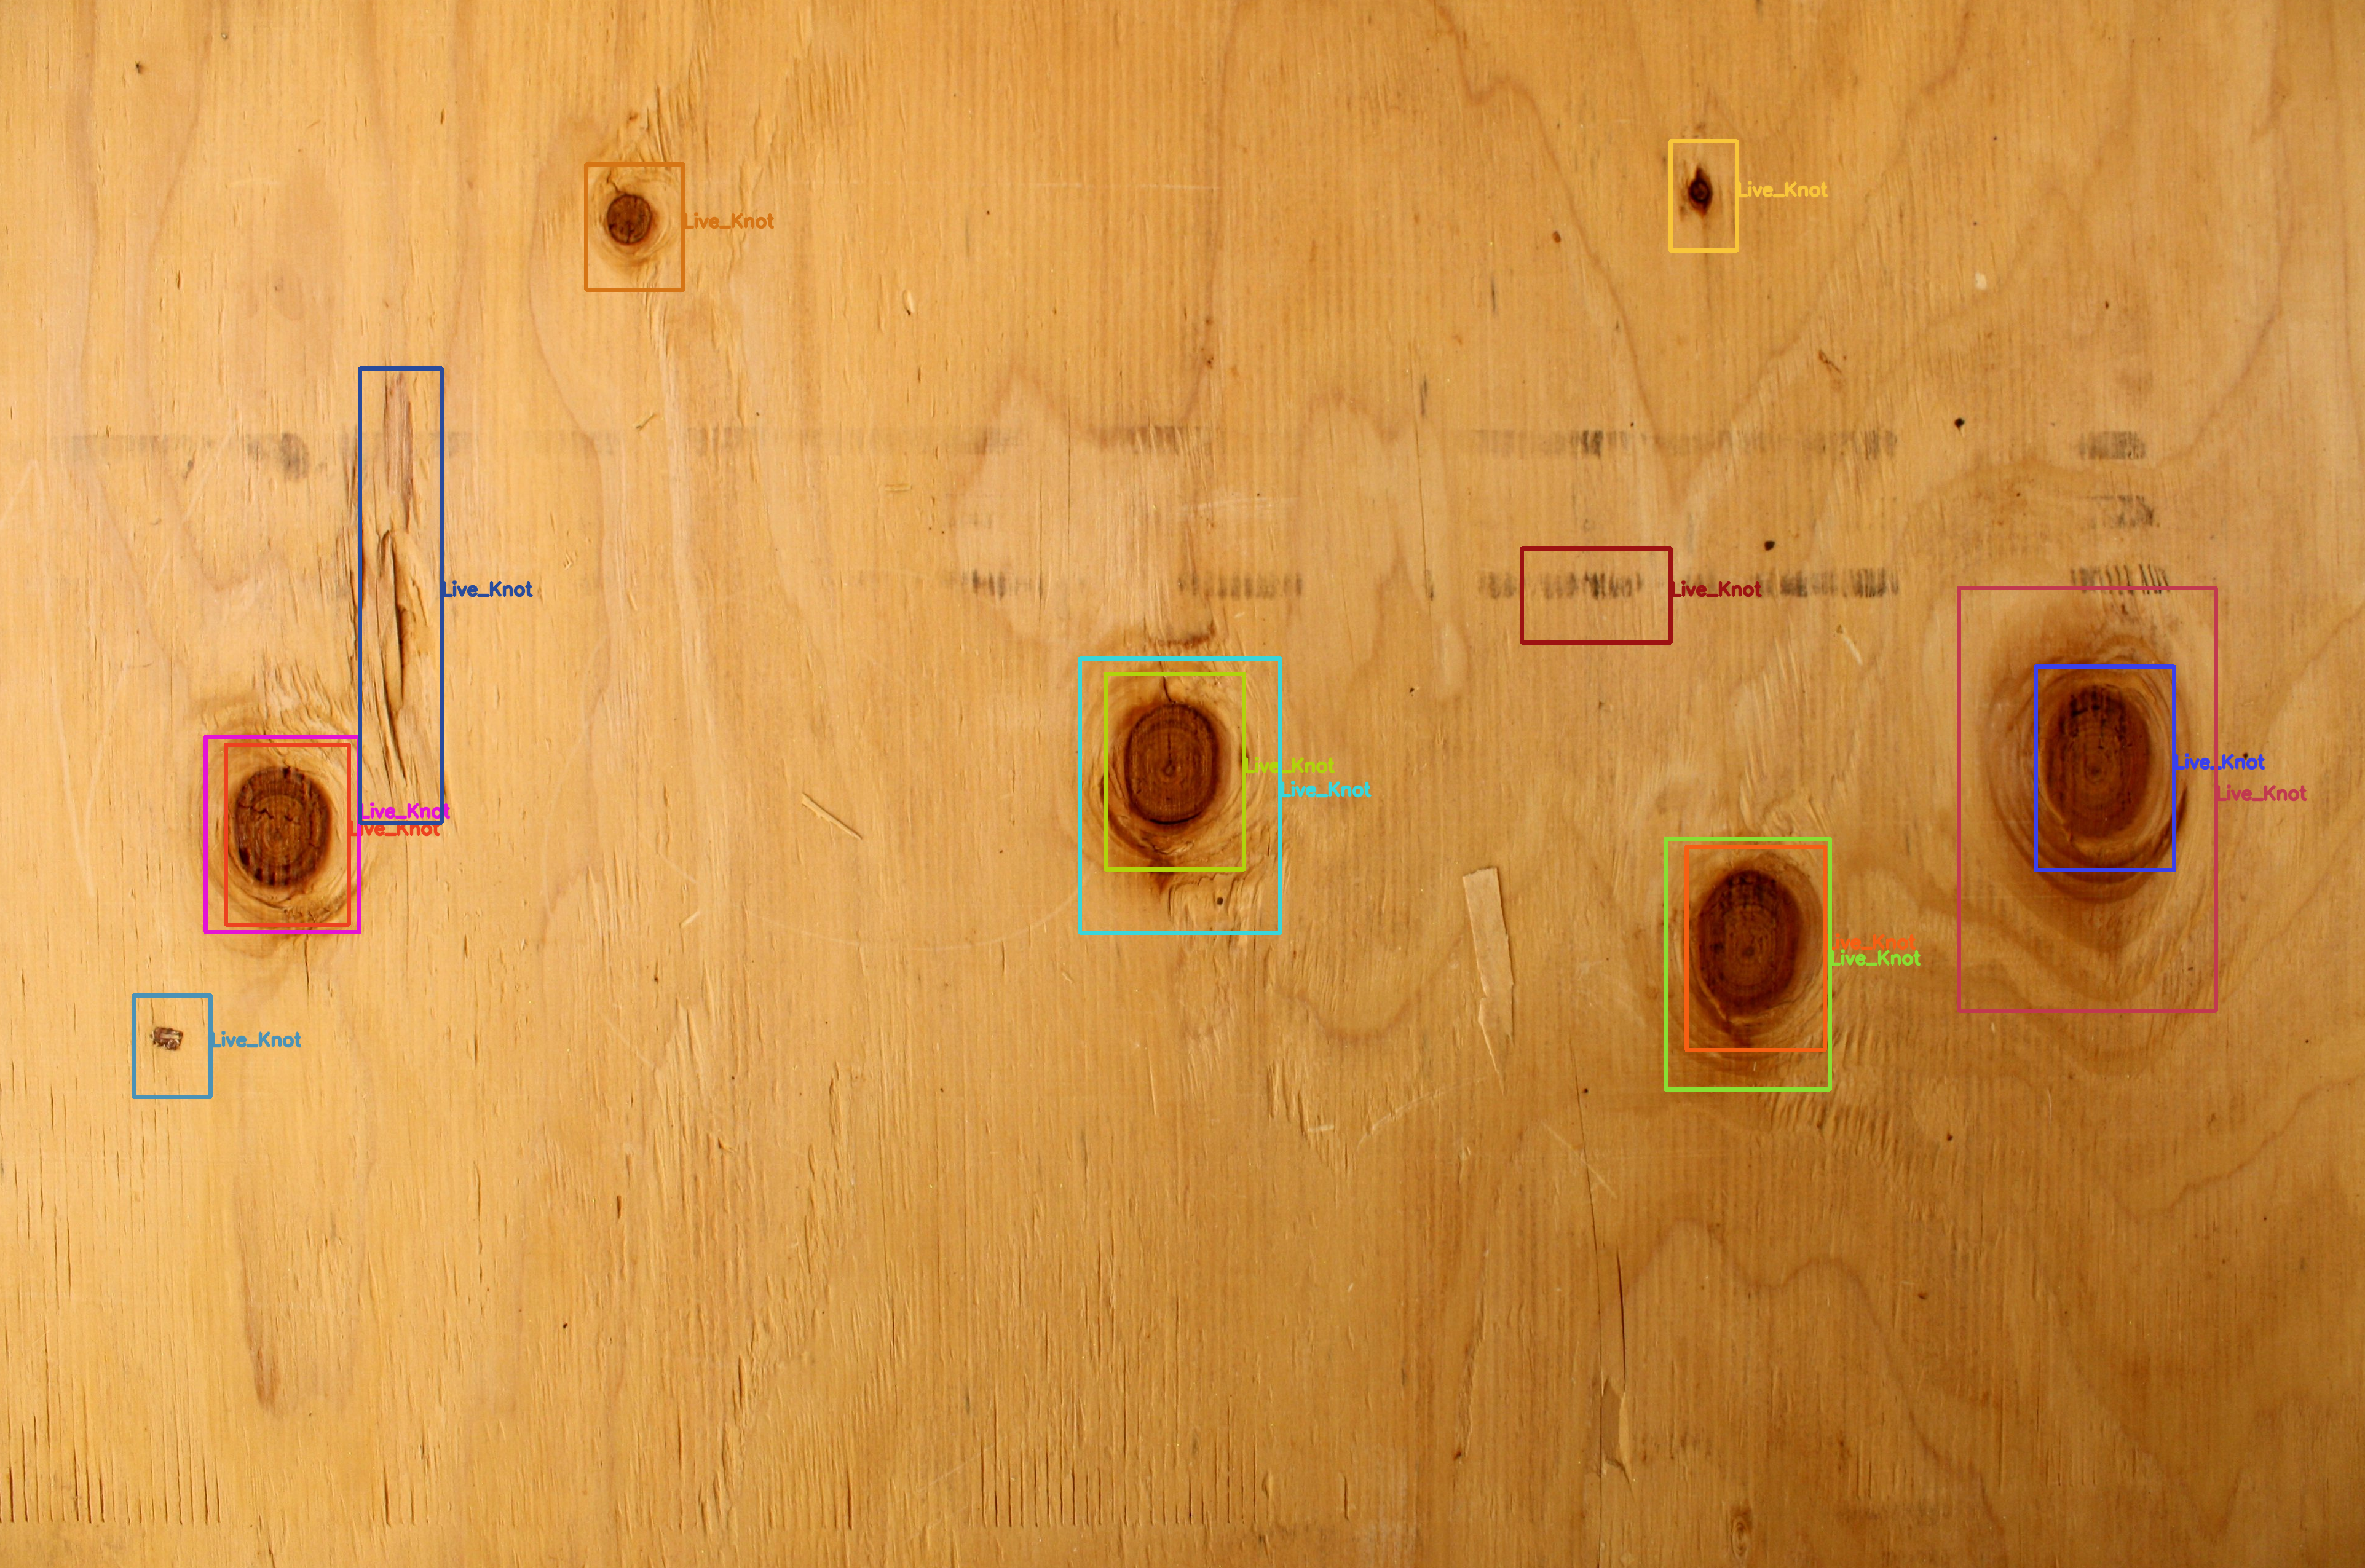
\includegraphics[width=0.5\textwidth]{3}}
			\caption{Метод Якобі (а), метод Зейделя (б), файл даних (в)}
		\end{figure}
		
		\section*{Висновок}
			На лабораторній роботі я засвоїв практичні навички використання методу Якобі та методу Зейделя та розробив функції для розв’язку системи лінійних алгебраїчних рівнянь 
			\begin{gather}\nonumber
				\left\{\begin{array}{@{}l@{}}
					0.65x_1-0.06x_2-0.12x_3+0.14x_4=2.17\\\nonumber
					0.04x_1-0.82x_2+0.08x_3+0.11x_4=-1.14\\\nonumber
					0.34x_1+0.08x_2-0.66x_3+0.14x_4=2.1\\\nonumber
					0.11x_1+0.12x_2\hspace{48pt}-0.53x_4=-0.58\nonumber
				\end{array}\right.\,
			\end{gather}
			за допомогою цих методів з точністю $\epsilon=0.001$. Корені системи рівнянь: $2.85; 1.70; -1.06; 2.07$. В результаті виконання програми видно, що кількість ітерацій методу Зейделя менша ніж методу Якобі.
	\end{large}
\end{document}
